\documentclass{article} 
\usepackage{amsmath}
\usepackage{amssymb}
\setlength{\parindent}{0pt}

\usepackage{graphicx}
\usepackage[a4paper, left=1.5in, right=1.5in, top=1.5in, bottom=1.5in]{geometry}
\usepackage{xcolor}

\usepackage{pgfplots}
\usetikzlibrary{intersections,angles,quotes}
\usepgfplotslibrary{fillbetween}
%\pgfplotsset{compat=1.17}
\begin{document}

\title{my review}
\maketitle

\textbf{calculus is a branch of mathematics that deals with rates of change and the accumulation of quantities.}

\section*{precalculus $\rightarrow$ calculus II}

$\lvert a\rvert = \lvert -a\rvert$, $\lvert ab\rvert = \lvert a\rvert\lvert b\rvert$\\

The \textbf{distance} between two real numbers $a$ and $b$ is $\lvert b - a \rvert$, which is the length of the line segment joining $a$ and $b$.\\
Two real numbers $a$ and $b$ are close to each other if $\lvert b - a\rvert$ is small, and this is the case if their decimal expansions agree to many places. More precisely, \textit{if the decimal expansions of a and b agree to k places (to the right of the decimal point), then the distance $\lvert b - a\rvert$ is at most $10^-k$. Thus, the distance between a = 3.1415 and b = 3.1478 is at most $10^{-2}$ because a and b agree to two places. In fact, the distance is exactly $\lvert3.1415 - 3.1478\rvert = 0.0063$.}\\

Beware that $\lvert a + b\rvert$ is not equal to $\lvert a\rvert + \lvert b\rvert$ unless $a$ and $b$ have the same sign or at least one of $a$ and $b$ is zero. If they have opposite sins, cancellation occurs in the sum $a + b$ and $\lvert a+b\rvert < \lvert a\rvert + \lvert b\rvert$. For example, $\lvert 2 + 5\rvert = \lvert2\rvert + \lvert5\rvert$ but $\lvert-2 + 5\rvert = 3$, which is less than $\lvert-2\rvert + \lvert5\rvert = 7$. In any case, $\lvert a + b\rvert$ is never larger than $\lvert a\rvert + \lvert b\rvert$ and this gives us the simple but important \textbf{trianlge inequality}: $\lvert a + b\rvert \leq \lvert a\rvert + \lvert b\rvert$\\

$[a, b] = {x \in \mathbb{R} : a \leq x \leq b}$\\
$(a, b) = {x \in \mathbb{R} : a < x < b}$\\
$[a, b) = {x \in \mathbb{R} : a \leq x < b}$\\
$(a, b] = {x \in \mathbb{R} : a < x \leq b}$\\

$(-r, r) = {x : \lvert x\rvert < r}$\\

circle: $(x-a)^2 + (y-b)^2 = r^2$ where $(a, b)$ is the center and the radius is $r$\\

midpoint between $P_1 = (x_1, y_1)$ and $P_2 = (x_2, y_2)$ is $\bar{P_{1}P_2}$ divided by 2\\

distance: $\sqrt{(x_2 - x_1)^2 + (y_2 - y_1)^2}$\\

laws of exponents: 

	\begin{itemize}
		\item $x^mx^n = x^{m+n}$
		\item $\frac{x^m}{x^n} = x^{m-n}$
		\item $(x^m)^n = x^{mn}$
		\item $x^{-n} = \frac{1}{x^n}$
		\item $(xy)^n = x^ny^n$
		\item $(\frac{x}{y})^n = \frac{x^n}{y^n}$
		\item $x^{1/n} = \sqrt[n]{x}$
		\item $x^{\frac{m}{n}} = \sqrt[n]{x^m} = (\sqrt[n]{x})^m$
	\end{itemize}

special factorizations

	\begin{itemize}
		\item $x^2 - y^2 = (x + y)(x - y)$
		\item $x^3 + y^3 = (x + y)(x^2 - xy + y^2)$
		\item $x^3 - y^3 = (x - y)(x^2 + xy + y^2)$
	\end{itemize}

binomial theorem:

	\begin{itemize}
		\item $(x + y)^2 = x^2 + 2xy + y^2$
		\item $(x - y)^2 = x^2 - 2xy + y^2$
		\item $(x + y)^3 = x^3 + 3x^2y + 3xy^2 + y^3$
		\item $(x - y)^3 = x^3 - 3x^2y + 3xy^2 - y^3$
		\item $(x + y)^n = x^n + nx^{n-1}y + \frac{n(n-1)}{2}x^{n-2}y^2 + \ldots + \binom{n}{k}x^{n-k}y^k + \dots + nxy^{n-1} + y^n$
			where $\binom{n}{k} = \frac{n(n-1) \dots (n-k+1)}{1 \cdot 2 \cdot 3 \cdot \ldots \cdot k}$
	\end{itemize}

quadratic formulae:

	\begin{enumerate}
		\item $ax^2 + bx + c = 0$
		\item $x^2 + \frac{b}{a}x + \frac{c}{a} = 0$
		\item $x^2 + \frac{b}{a}x = -\frac{c}{a}$
		\item $x^2 + \frac{b}{a}x + \left( \frac{b}{2a} \right)^2 = -\frac{c}{a} + \left( \frac{b}{2a} \right)^2$
		\item $\left( x + \frac{b}{2a} \right)^2 = \frac{b^2 - 4ac}{4a^2}$
		\item $x + \frac{b}{2a} = \pm \frac{\sqrt{b^2 - 4ac}}{2a}$
		\item $x = -\frac{b}{2a} \pm \frac{\sqrt{b^2 - 4ac}}{2a}$
		\item $x = \frac{-b \pm \sqrt{b^2 - 4ac}}{2a}$
	\end{enumerate}

polynomials $a_nx^n + a_{n-1}x^{n-1} + ... + a_1x + a_0$ where n is non-neg and represents the degree\\

rational $p(x)/q(x)$\\

root $\sqrt[n]{g(x)}$\\

properties:\\
	domain: set of all input values for which the function is defined\\
	range: set of all possible output values of the function\\
	
	continuity: most algebaic functions are continuous (no breaks of jumps), but rational functions have discontinuities at points\\
		
	behavior: the functions behavior is influenced by the degree of the polynomial and the nature of the function\\


	scaling:
		\begin{itemize}
			\item{vertical scaling} $y = kf(x)$: If $k \geq 1$, the graph is expanded vertically by the factor $k$. If $0 < k < 1$, the graph is compressed vertically. When the scale factor $k$ is negative $(k < 0)$, the graph is also reflected across the x-axis.
			\item{horizontal scaling} $y = f(kx)$: If $K \geq 1$, the graph is compressed in the horizontal direction. If $0 < k < 1$, the graph is expanded. If $k \leq 0$, then the graph is also reflected across the y-axis.
		\end{itemize}

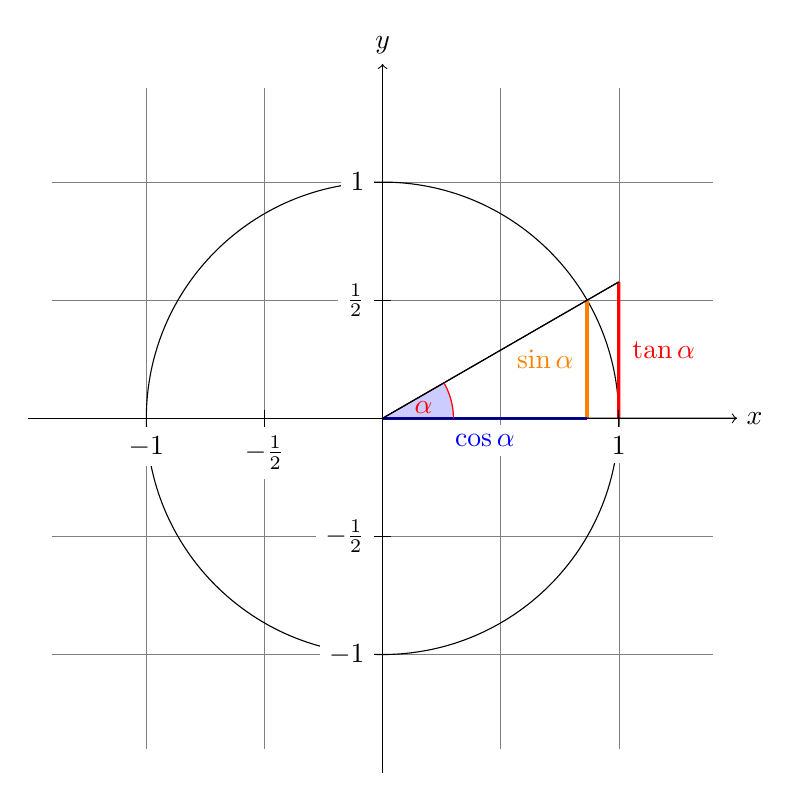
\begin{tikzpicture}[scale=3]

%grid lines
\draw[
        step=.5cm,
        gray,
        very thin
        ] 
        (-1.4,-1.4) grid (1.4,1.4);
\filldraw[
            fill=blue!20,
            draw=red!50
            ] 
            (0,0) -- (3mm,0mm)
arc [
        start angle=0, 
        end angle=30, 
        radius=3mm] 
        -- cycle;
%axes
\draw[->] (-1.5,0) -- (1.5,0) coordinate (x axis);
\draw[->] (0,-1.5) -- (0,1.5) coordinate (y axis);

%axes label
\node [right]at (1.5,0)(x){$x$};    
\node [above]at (0,1.5){$y$};

%circle 
\draw (0,0) circle [
                    radius=1cm
                    ];
                    
%triangle height
\draw[
        very thick,
        orange
        ]
        (30:1cm) -- node[
                        left=1pt,
                        fill=white
                        ] 
                        {$\sin \alpha$} (30:1cm |- x axis);
                        
%triangle base
\draw[
        very thick,
        blue
        ]
        (30:1cm |- x axis) -- node[
                                    below=2pt,
                                    fill=white
                                    ] 
                                    {$\cos \alpha$} (0,0);

%intersection
\path [name path=upward line] (1,0) -- (1,1);
\path [name path=sloped line] (0,0) -- (30:1.5cm);
\draw [name intersections={of=upward line and sloped line, by=t}]
        [very thick,red] 
        (1,0) -- node [right=1pt,fill=white]
        {$\displaystyle \tan \alpha $} (t);
\draw (0,0) -- (t);

%x-ticks
\foreach \x/\xtext in {-1, 
                        -0.5/-\frac{1}{2},
                                         1}
\draw (\x cm,1pt) -- (\x cm,-1pt) node[
                                        anchor=north,
                                        fill=white
                                        ] 
                                        {$\xtext$};
%y-ticks
\foreach \y/\ytext in {-1, 
                        -0.5/-\frac{1}{2}, 
                            0.5/\frac{1}{2}, 
                                            1}
\draw (1pt,\y cm) -- (-1pt,\y cm) node[
                                        anchor=east,
                                        fill=white
                                        ] 
                                        {$\ytext$};
%arc angle
\draw (x) coordinate (A)-- 
        (0,0) coordinate (B)-- 
            (t) coordinate (C)
pic [
        draw,
        red, 
        "$\alpha$",
        angle radius=9mm
        ] 
        {angle};
\end{tikzpicture}
\\
\\
\\
$
\begin{array}{|c|c|c|c|}
\hline
\text{Angle (Degrees)} & \text{Angle (Radians)} & \cos(\theta) & \sin(\theta) \\
\hline
0^\circ & 0 & 1 & 0 \\
30^\circ & \frac{\pi}{6} & \frac{\sqrt{3}}{2} & \frac{1}{2} \\
45^\circ & \frac{\pi}{4} & \frac{\sqrt{2}}{2} & \frac{\sqrt{2}}{2} \\
60^\circ & \frac{\pi}{3} & \frac{1}{2} & \frac{\sqrt{3}}{2} \\
90^\circ & \frac{\pi}{2} & 0 & 1 \\
\hline
120^\circ & \frac{2\pi}{3} & -\frac{1}{2} & \frac{\sqrt{3}}{2} \\
135^\circ & \frac{3\pi}{4} & -\frac{\sqrt{2}}{2} & \frac{\sqrt{2}}{2} \\
150^\circ & \frac{5\pi}{6} & -\frac{\sqrt{3}}{2} & \frac{1}{2} \\
180^\circ & \pi & -1 & 0 \\
\hline
210^\circ & \frac{7\pi}{6} & -\frac{\sqrt{3}}{2} & -\frac{1}{2} \\
225^\circ & \frac{5\pi}{4} & -\frac{\sqrt{2}}{2} & -\frac{\sqrt{2}}{2} \\
240^\circ & \frac{4\pi}{3} & -\frac{1}{2} & -\frac{\sqrt{3}}{2} \\
270^\circ & \frac{3\pi}{2} & 0 & -1 \\
\hline
300^\circ & \frac{5\pi}{3} & \frac{1}{2} & -\frac{\sqrt{3}}{2} \\
315^\circ & \frac{7\pi}{4} & \frac{\sqrt{2}}{2} & -\frac{\sqrt{2}}{2} \\
330^\circ & \frac{11\pi}{6} & \frac{\sqrt{3}}{2} & -\frac{1}{2} \\
360^\circ & 2\pi & 1 & 0 \\
\hline
\end{array}
$
\\
\\
\\

$1^\circ = \frac{\pi}{180}$rad\\

$1 rad = \frac{180^\circ}{pi}$\\

\textbf{SOH-CAH-TOA} is a mnemonic device that expresses the relationship between the basic trigonometric functions and the ratios of the sides in a right triangle.\\

trigonometric functions are mathematical functions that relate the angle of a trianlge to the lengths of its sides... and can also be generalized to all real numbers using the unit circle.\\

To derive the rest of the fundamental trigonometric identities, you need a combination of a few key identities and principles. The most important starting point is the Pythagorean identity, but you’ll also need the basic relationships between the trigonometric functions, such as the definitions of sine, cosine, tangent, secant, cosecant, and cotangent in terms of a right triangle or the unit circle. \\

$ \sin^2 \theta + \cos^2 \theta = 1 $\\

$ \sec \theta = \frac{1}{\cos \theta}, \quad \csc \theta = \frac{1}{\sin \theta}, \quad \cot \theta = \frac{1}{\tan \theta} $\\

$ \tan \theta = \frac{\sin \theta}{\cos \theta}, \quad \cot \theta = \frac{\cos \theta}{\sin \theta} $\\

$ 1 + \tan^2 \theta = \sec^2 \theta $\\

$ 1 + \cot^2 \theta = \csc^2 \theta $\\

$ \sin(\alpha + \beta) = \sin \alpha \cos \beta + \cos \alpha \sin \beta $\\

$ \cos(\alpha + \beta) = \cos \alpha \cos \beta - \sin \alpha \sin \beta $\\

$ \tan(\alpha + \beta) = \frac{\tan \alpha + \tan \beta}{1 - \tan \alpha \tan \beta} $\\

$ \sin(\alpha - \beta) = \sin \alpha \cos \beta - \cos \alpha \sin \beta $\\

$ \cos(\alpha - \beta) = \cos \alpha \cos \beta + \sin \alpha \sin \beta $\\

$ \tan(\alpha - \beta) = \frac{\tan \alpha - \tan \beta}{1 + \tan \alpha \tan \beta} $\\

$ \sin(2\theta) = 2\sin \theta \cos \theta $\\

$ \cos(2\theta) = \cos^2 \theta - \sin^2 \theta = 2\cos^2 \theta - 1 = 1 - 2\sin^2 \theta $\\

$ \tan(2\theta) = \frac{2\tan \theta}{1 - \tan^2 \theta} $\\

$ \sin^2(2\theta) = \frac{1 - \cos^2(2\theta)}{2} $\\

$ \cos^2(2\theta) = \frac{1 + \cos(2\theta)}{2} $\\

$ \sin(90^\circ - \theta) = \cos \theta, \quad \cos(90^\circ - \theta) = \sin \theta $\\

$ \tan(90^\circ - \theta) = \cot \theta, \quad \cot(90^\circ - \theta) = \tan \theta $\\

$ \sec(90^\circ - \theta) = \csc \theta, \quad \csc(90^\circ - \theta) = \sec \theta $\\

$ \sin(-\theta) = -\sin(\theta), \quad \cos(-\theta) = \cos(\theta) $\\

$ \tan(-\theta) = -\tan(\theta), \quad \sec(-\theta) = \sec(\theta) $\\

$ \csc(-\theta) = -\csc(\theta), \quad \cot(-\theta) = -\cot(\theta) $\\

$ \sin \alpha \sin \beta = \frac{1}{2} [\cos(\alpha - \beta) - \cos(\alpha + \beta)] $\\

$ \cos \alpha \cos \beta = \frac{1}{2} [\cos(\alpha - \beta) + \cos(\alpha + \beta)] $\\

$ \sin \alpha \cos \beta = \frac{1}{2} [\sin(\alpha + \beta) + \sin(\alpha - \beta)] $\\

law of sines: $ \frac{\sin(A)}{a} = \frac{\sin(B)}{b} = \frac{\sin(C)}{c} $ (uppercase are the angles)\\

law of cosines: $ a^2 = b^2+c^2 - 2bc\cos(A) $\\

power functions: $f(x) = x^n$....if even the function behaves symmetrical around the y-axis...if odd then the function has point symmetry ($x^4$, $x^3$, $x^{-n} = \frac{1}{x^n}$)\\

inverse trig functions: $\arcsin(x) = \sin^{-1}(x) = \theta$, $\arccos(x) = \cos^{-1}(x) = \theta$...etc\\

logs: $\log_ax=y \leftrightarrow a^y = x$, $\ln(x)=y \leftrightarrow e^y=x$\\

hyperbolic functions: $\sinh(x) = \frac{e^x-e^{-x}}{2}$, $\cosh(x) = \frac{e^x+e^{-x}}{2}$, $\tanh(x) = \frac{\sinh(x)}{\cosh(x)}$\\

differentiation rules:
	\begin{enumerate}
		\item$\frac{d}{dx}(c) = 0$
		\item$\frac{d}{dx}x = 1$
		\item$\frac{d}{dx}(x^n) = nx^{-1}$ (power rule)
		\item$\frac{d}{dx}[cf(x)] = cf'(x)$
		\item$\frac{d}{dx}[f(x)+g(x)] = f'(x) + g'(x)$
		\item$\frac{d}{dx}[f(x)g(x)] = f(x)g'(x) + g(x)f'(x)$ (product rule)
		\item$\frac{d}{dx}[\frac{f(x)}{g(x)}] = \frac{g(x)f'(x) - f(x)g'(x)}{[g(x)]^2}$ (quotient rule)
		\item$\frac{d}{dx}f(g(x)) = f'(g(x))g'(x)$ (chain rule)
		\item$\frac{d}{dx}f(x)^n = nf(x)^{n-1}f'(x)$ (general power rule)
		\item$\frac{d}{dx}\sin(x) = \cos(x)$ 
		\item$\frac{d}{dx}\cos(x) = -\sin(x)$
		\item$\frac{d}{dx}\tan(x) = \sec^2(x)$
		\item$\frac{d}{dx}\csc(x) = -\csc(x)\cot(x)$
		\item$\frac{d}{dx}\sec(x) = \sec(x)\tan(x)$
		\item$\frac{d}{dx}\cot(x) = -\csc^2(x)$
		\item$\frac{d}{dx}\sin^{-1}(x) = \frac{1}{\sqrt(1 - x^2)}$
		\item$\frac{d}{dx}\cos^{-1}(x) = -\frac{1}{\sqrt(1 - x^2)}$
		\item$\frac{d}{dx}\tan^{-1}(x) = \frac{1}{1 + x^2}$
		\item$\frac{d}{dx}(e^x) = e^x$
		\item$\frac{d}{dx}(a^x) (\ln a)a^x$
		\item$\frac{d}{dx}\ln\mid x\mid = \frac{1}{x}$
		\item$\frac{d}{dx}\log_ax = \frac{1}{(\ln a)x}$
	\end{enumerate}


Essential Theorems:
\begin{itemize}
    \item \textbf{Intermediate Value Theorem (IVT):} Guarantees that a continuous function takes every value between \( f(a) \) and \( f(b) \) at some point in the interval \([a, b]\).
    \item \textbf{Mean Value Theorem (MVT):} States that for a continuous and differentiable function, there is at least one point where the instantaneous rate of change equals the average rate of change over the interval.
    \item \textbf{Extreme Value Theorem:} Guarantees that a continuous function on a closed interval attains a maximum and minimum value.
    \item \textbf{Fundamental Theorem of Calculus:}
    \begin{enumerate}
        \item \textbf{First Part:} The derivative of the integral of a function is the original function.
        \item \textbf{Second Part:} The definite integral of a function can be computed using its antiderivative.
    \end{enumerate}
\end{itemize}

\newpage
\section*{review problems}

verifying trigonometric identities:
	\begin{enumerate}
		\item $\frac{1 + \sin(x)}{\cos(x)} + \frac{1 - \sin(x)}{\cos(x)} = 2\sec(x)$
		\item $\frac{\sin(x)}{1 + \cos(x)} + \frac{\sin(x)}{1 - \cos(x)} = \frac{2\sin(x)}{1 - \cos^2(x)}$
		\item $\frac{\tan(x) + \cot(x)}{\sec(x) + \csc(x)} = \sin(x)\cos(x)$
		\item $\frac{\sin(x) - \cos(x)}{\sin(x) + \cos(x)} = \frac{1 - \tan(x)}{1 + \tan(x)}$
		\item $\frac{1 - \cos(2x)}{2\sin(x)\cos(x)} = \tan(x)$
	\end{enumerate}

solving trigonometric equations:\\
bounded:
\begin{enumerate}
	\item $ \sin(x) = \frac{1}{2} \quad \text{for } 0 \leq x < 2\pi $  
	\item $ 2\cos(x) - 1 = 0 \quad \text{for } 0 \leq x < 2\pi $ 
	\item $ \sin^2(x) - \sin(x) = 0 \quad \text{for } 0 \leq x < 2\pi $ 
	\item $ 2\cos^2(x) - 3\cos(x) + 1 = 0 \quad \text{for } 0 \leq x < 2\pi $ 
	\item $ \sin(x)\cos(x) = \frac{1}{2} \quad \text{for } 0 \leq x < 2\pi $ 
	\item $ \tan(x) + \cot(x) = 2 \quad \text{for } 0 < x < \pi $ 
	\item $ 1 - 2\sin^2(x) = \cos(2x) \quad \text{for } 0 \leq x < 2\pi $ 
	\item $ \sec(x) = 2 \quad \text{for } 0 \leq x < 2\pi $ 
	\item $ \sin(2x) = \sqrt{3}\cos(x) \quad \text{for } 0 \leq x < 2\pi $
	\item $ \tan^2(x) = 3 \quad \text{for } 0 \leq x < 2\pi $
\end{enumerate}
unbounded:
\begin{enumerate}
  \item $\sin(x)=\frac{1}{2}$
  \item $\cos(x)=-\frac{\sqrt{2}}{2}$
  \item $\tan(x)=\sqrt{3}$
  \item $2\sin(x)-1=0$
  \item $\cos^2(x)=\frac{1}{4}$
  \item $\sec(x)=-2$
  \item $\tan^2(x)=1$
  \item $\cot(x)+1=0$
  \item $\sin(2x)=0$
  \item $\cos(3x)=1$
\end{enumerate}

direct substitution:
\begin{enumerate}
	\item $\lim_{x \to 3} \left( 2x^2 - 5x + 4 \right)$
	\item $\lim_{x \to 0} \left( \frac{3x^2 + 2x - 1}{x + 2} \right)$
        \item $\lim_{x \to -1} \left( 4x^3 - 2x + 6 \right)$
	\item $\lim_{x \to 2} \left( \frac{x^2 - 4}{x - 2} \right)$
	\item $\lim_{x \to 1} \left( 3x^3 - 2x + 5 \right)$
	\item $\lim_{x \to 0} \left( \frac{5x^2 + 3x}{x^2 + 2x + 1} \right)$
	\item $\lim_{x \to 4} \left( \sqrt{x} - 2 \right)$
	\item $\lim_{x \to 0} \left( \frac{x^3 + 2x}{x^2 - 3x + 2} \right)$
	\item $\lim_{x \to 1} \left( \frac{x^2 + x - 2}{x - 1} \right)$
	\item $\lim_{x \to -3} \left( \frac{2x + 1}{x^2 + 5x + 6} \right)$
\end{enumerate}

indeterminate forms and algebraic simplification
\begin{enumerate}
        \item $\lim_{x \to 2} \frac{x^2 - 4}{x - 2}$
        \item $\lim_{x \to 0} \frac{\sin(x)}{x}$
        \item $\lim_{x \to 0} \frac{e^x - 1}{x}$
        \item $\lim_{x \to 0} \frac{1 - \cos(x)}{x^2}$
        \item $\lim_{x \to 0} \frac{x^2 + 3x}{x}$
        \item $\lim_{x \to 1} \frac{x^3 - 1}{x - 1}$
        \item $\lim_{x \to \infty} \frac{1}{x}$
        \item $\lim_{x \to 0} \frac{\ln(x)}{x}$
        \item $\lim_{x \to 0} \frac{x^2 + 2x - 3}{x^2 - 1}$
        \item $\lim_{x \to 0} \frac{x^3 + x}{x^2 - 1}$
\end{enumerate}

trigonometic limits:
\begin{enumerate}
        \item $\lim_{x \to 0} \frac{\sin(x)}{x}$
        \item $\lim_{x \to 0} \frac{1 - \cos(x)}{x^2}$
        \item $\lim_{x \to 0} \frac{\tan(x)}{x}$
        \item $\lim_{x \to 0} \frac{\sin(3x)}{x}$
        \item $\lim_{x \to 0} \frac{1 - \cos(2x)}{x^2}$
        \item $\lim_{x \to 0} \frac{\sin(x) - \sin(2x)}{x}$
        \item $\lim_{x \to \infty} \frac{\sin(x)}{x}$
        \item $\lim_{x \to 0} \frac{\cos(x) - 1}{x^2}$
        \item $\lim_{x \to 0} \frac{\sin(x)}{x^3}$
        \item $\lim_{x \to 0} \frac{\tan(2x)}{x}$
\end{enumerate}

piecewise functions:
\begin{enumerate}
        \item $\lim_{x \to 0} \left\{ \begin{array}{ll} 
        \sin(x) & \text{if } x \geq 0 \\
        -\sin(x) & \text{if } x < 0 \end{array} \right.$
        \item $\lim_{x \to 0} \left\{ \begin{array}{ll} 
        \frac{x^2 - 4}{x - 2} & \text{if } x \neq 2 \\
        4 & \text{if } x = 2 \end{array} \right.$
        \item $\lim_{x \to 0} \left\{ \begin{array}{ll} 
        \frac{\sin(x)}{x} & \text{if } x \neq 0 \\
        1 & \text{if } x = 0 \end{array} \right.$
        \item $\lim_{x \to \pi} \left\{ \begin{array}{ll} 
        \cos(x) & \text{if } x < \pi \\
        \sin(x) & \text{if } x \geq \pi \end{array} \right.$
        \item $\lim_{x \to 0} \left\{ \begin{array}{ll} 
        \frac{\sin(2x)}{x} & \text{if } x \neq 0 \\
        0 & \text{if } x = 0 \end{array} \right.$
        \item $\lim_{x \to 0} \left\{ \begin{array}{ll} 
        \frac{1 - \cos(x)}{x} & \text{if } x \neq 0 \\
        0 & \text{if } x = 0 \end{array} \right.$
        \item $\lim_{x \to 0} \left\{ \begin{array}{ll} 
        \tan(x) & \text{if } x \geq 0 \\
        -\tan(x) & \text{if } x < 0 \end{array} \right.$
        \item $\lim_{x \to 0} \left\{ \begin{array}{ll} 
        \frac{\sin(x) - \sin(2x)}{x} & \text{if } x \neq 0 \\
        0 & \text{if } x = 0 \end{array} \right.$
        \item $\lim_{x \to 0} \left\{ \begin{array}{ll} 
        \frac{\sin(3x)}{x} & \text{if } x \neq 0 \\
        3 & \text{if } x = 0 \end{array} \right.$
        \item $\lim_{x \to 0} \left\{ \begin{array}{ll} 
        \frac{x^2}{\sin(x)} & \text{if } x \neq 0 \\
        0 & \text{if } x = 0 \end{array} \right.$
\end{enumerate}

infinite limits and vertical asymptotes:
\begin{enumerate}
        \item $\lim_{x \to 0^+} \frac{1}{x}$
        \item $\lim_{x \to 0^-} \frac{1}{x}$
        \item $\lim_{x \to \infty} \frac{1}{x^2}$
        \item $\lim_{x \to 0} \frac{1}{x^2}$
        \item $\lim_{x \to 2^+} \frac{1}{x-2}$
        \item $\lim_{x \to -2^-} \frac{1}{x+2}$
        \item $\lim_{x \to 0^+} \frac{\ln(x)}{x}$
        \item $\lim_{x \to \infty} \frac{x^2}{x+1}$
        \item $\lim_{x \to 3} \frac{1}{(x-3)^2}$
        \item $\lim_{x \to 1} \frac{1}{x-1}$
\end{enumerate}

squeeze theorem:
\begin{enumerate}
	\item
\end{enumerate}

epsilon-delta:
\begin{enumerate}
	\item
\end{enumerate}

basic polynomial differentiation:
\begin{enumerate}
        \item Differentiate $f(x) = 3x^4 + 5x^3 - 2x + 7$
        \item Differentiate $f(x) = 4x^5 - x^2 + 6x - 3$
        \item Differentiate $f(x) = x^6 + 2x^4 - 3x^2 + x - 8$
        \item Differentiate $f(x) = 5x^3 - 4x^2 + 7x + 1$
        \item Differentiate $f(x) = 2x^5 - x^3 + x - 9$
        \item Differentiate $f(x) = 3x^2 - 2x + 4$
        \item Differentiate $f(x) = x^7 - 5x^3 + 2x^2 - x + 6$
        \item Differentiate $f(x) = 6x^4 - 3x^3 + 2x^2 + x - 5$
        \item Differentiate $f(x) = 2x^8 - x^6 + 4x^2 - 3$
        \item Differentiate $f(x) = 9x^5 - 7x^4 + 3x^2 + 2x + 1$
\end{enumerate}

implicit differentiation:
\begin{enumerate}
        \item Differentiate $x^2 + y^2 = 25$
        \item Differentiate $x^3 + y^3 = 6xy$
        \item Differentiate $x^2y + y^2 = 10$
        \item Differentiate $x^2 + 2xy + y^2 = 7$
        \item Differentiate $x^3 + y^3 = 3xy$
        \item Differentiate $x^2y^2 + 3x = 5$
        \item Differentiate $x^2 + y^2 = x + y$
        \item Differentiate $x^3 + y^3 = 6x + 2y$
        \item Differentiate $xy = x + y$
        \item Differentiate $x^2 - 3xy + y^2 = 10$
\end{enumerate}

higher-order derivatives:
\begin{enumerate}
        \item Find the second derivative of $f(x) = 3x^4 - 5x^2 + 2x - 7$
        \item Find the third derivative of $f(x) = x^5 - 3x^3 + 4x^2 - 6$
        \item Find the second derivative of $f(x) = \sin(x) + \cos(x)$
        \item Find the first and second derivatives of $f(x) = e^{2x} \cos(x)$
        \item Find the third derivative of $f(x) = 4x^3 + 3x^2 - 2x + 5$
        \item Find the first and second derivatives of $f(x) = \ln(x^2 + 1)$
        \item Find the second derivative of $f(x) = \tan(x)$
        \item Find the fourth derivative of $f(x) = 7x^4 - 6x^2 + x - 3$
        \item Find the second derivative of $f(x) = \frac{x^3}{x^2 + 1}$
        \item Find the third derivative of $f(x) = x^4 \ln(x)$
\end{enumerate}

applications of derivatives (tangent line equations, critical points, motion problems, related rates):

basic antiderivatives:

u-sub (reverse chain rule):

trig integrals:

integration by parts:

partial fractions:

applications (area under curves, average value of a function, volume by disks/washers/shells, accumulation problems):

\end{document}
